\documentclass[twoside]{book}

% Packages required by doxygen
\usepackage{fixltx2e}
\usepackage{calc}
\usepackage{doxygen}
\usepackage[export]{adjustbox} % also loads graphicx
\usepackage{graphicx}
\usepackage[utf8]{inputenc}
\usepackage{makeidx}
\usepackage{multicol}
\usepackage{multirow}
\PassOptionsToPackage{warn}{textcomp}
\usepackage{textcomp}
\usepackage[nointegrals]{wasysym}
\usepackage[table]{xcolor}

% Font selection
\usepackage[T1]{fontenc}
\usepackage[scaled=.90]{helvet}
\usepackage{courier}
\usepackage{amssymb}
\usepackage{sectsty}
\renewcommand{\familydefault}{\sfdefault}
\allsectionsfont{%
  \fontseries{bc}\selectfont%
  \color{darkgray}%
}
\renewcommand{\DoxyLabelFont}{%
  \fontseries{bc}\selectfont%
  \color{darkgray}%
}
\newcommand{\+}{\discretionary{\mbox{\scriptsize$\hookleftarrow$}}{}{}}

% Page & text layout
\usepackage{geometry}
\geometry{%
  a4paper,%
  top=2.5cm,%
  bottom=2.5cm,%
  left=2.5cm,%
  right=2.5cm%
}
\tolerance=750
\hfuzz=15pt
\hbadness=750
\setlength{\emergencystretch}{15pt}
\setlength{\parindent}{0cm}
\setlength{\parskip}{3ex plus 2ex minus 2ex}
\makeatletter
\renewcommand{\paragraph}{%
  \@startsection{paragraph}{4}{0ex}{-1.0ex}{1.0ex}{%
    \normalfont\normalsize\bfseries\SS@parafont%
  }%
}
\renewcommand{\subparagraph}{%
  \@startsection{subparagraph}{5}{0ex}{-1.0ex}{1.0ex}{%
    \normalfont\normalsize\bfseries\SS@subparafont%
  }%
}
\makeatother

% Headers & footers
\usepackage{fancyhdr}
\pagestyle{fancyplain}
\fancyhead[LE]{\fancyplain{}{\bfseries\thepage}}
\fancyhead[CE]{\fancyplain{}{}}
\fancyhead[RE]{\fancyplain{}{\bfseries\leftmark}}
\fancyhead[LO]{\fancyplain{}{\bfseries\rightmark}}
\fancyhead[CO]{\fancyplain{}{}}
\fancyhead[RO]{\fancyplain{}{\bfseries\thepage}}
\fancyfoot[LE]{\fancyplain{}{}}
\fancyfoot[CE]{\fancyplain{}{}}
\fancyfoot[RE]{\fancyplain{}{\bfseries\scriptsize Generated by Doxygen }}
\fancyfoot[LO]{\fancyplain{}{\bfseries\scriptsize Generated by Doxygen }}
\fancyfoot[CO]{\fancyplain{}{}}
\fancyfoot[RO]{\fancyplain{}{}}
\renewcommand{\footrulewidth}{0.4pt}
\renewcommand{\chaptermark}[1]{%
  \markboth{#1}{}%
}
\renewcommand{\sectionmark}[1]{%
  \markright{\thesection\ #1}%
}

% Indices & bibliography
\usepackage{natbib}
\usepackage[titles]{tocloft}
\setcounter{tocdepth}{3}
\setcounter{secnumdepth}{5}
\makeindex

% Hyperlinks (required, but should be loaded last)
\usepackage{ifpdf}
\ifpdf
  \usepackage[pdftex,pagebackref=true]{hyperref}
\else
  \usepackage[ps2pdf,pagebackref=true]{hyperref}
\fi
\hypersetup{%
  colorlinks=true,%
  linkcolor=blue,%
  citecolor=blue,%
  unicode%
}

% Custom commands
\newcommand{\clearemptydoublepage}{%
  \newpage{\pagestyle{empty}\cleardoublepage}%
}

\usepackage{caption}
\captionsetup{labelsep=space,justification=centering,font={bf},singlelinecheck=off,skip=4pt,position=top}

%===== C O N T E N T S =====

\begin{document}

% Titlepage & ToC
\hypersetup{pageanchor=false,
             bookmarksnumbered=true,
             pdfencoding=unicode
            }
\pagenumbering{alph}
\begin{titlepage}
\vspace*{7cm}
\begin{center}%
{\Large Optimization \\[1ex]\large 1.\+0 v }\\
\vspace*{1cm}
{\large Generated by Doxygen 1.8.13}\\
\end{center}
\end{titlepage}
\clearemptydoublepage
\pagenumbering{roman}
\tableofcontents
\clearemptydoublepage
\pagenumbering{arabic}
\hypersetup{pageanchor=true}

%--- Begin generated contents ---
\chapter{Hierarchical Index}
\section{Class Hierarchy}
This inheritance list is sorted roughly, but not completely, alphabetically\+:\begin{DoxyCompactList}
\item \contentsline{section}{Abstract\+Area}{\pageref{class_abstract_area}}{}
\begin{DoxyCompactList}
\item \contentsline{section}{Square\+Area}{\pageref{class_square_area}}{}
\end{DoxyCompactList}
\item \contentsline{section}{Abstract\+Criterion}{\pageref{class_abstract_criterion}}{}
\begin{DoxyCompactList}
\item \contentsline{section}{Epsilon\+Criterion}{\pageref{class_epsilon_criterion}}{}
\item \contentsline{section}{Euclid\+Norm\+Criterion}{\pageref{class_euclid_norm_criterion}}{}
\end{DoxyCompactList}
\item \contentsline{section}{Abstract\+Optimization\+Method}{\pageref{class_abstract_optimization_method}}{}
\begin{DoxyCompactList}
\item \contentsline{section}{Nelder\+Mead\+Optimization}{\pageref{class_nelder_mead_optimization}}{}
\item \contentsline{section}{Random\+Search}{\pageref{class_random_search}}{}
\end{DoxyCompactList}
\item \contentsline{section}{Function}{\pageref{class_function}}{}
\begin{DoxyCompactList}
\item \contentsline{section}{Function\+Optimize}{\pageref{class_function_optimize}}{}
\end{DoxyCompactList}
\item \contentsline{section}{Optimization\+Result}{\pageref{class_optimization_result}}{}
\end{DoxyCompactList}

\chapter{Class Index}
\section{Class List}
Here are the classes, structs, unions and interfaces with brief descriptions\+:\begin{DoxyCompactList}
\item\contentsline{section}{\hyperlink{class_abstract_area}{Abstract\+Area} \\*Abstract base class for area }{\pageref{class_abstract_area}}{}
\item\contentsline{section}{\hyperlink{class_abstract_criterion}{Abstract\+Criterion} \\*Abstract base class for criterion of stopping }{\pageref{class_abstract_criterion}}{}
\item\contentsline{section}{\hyperlink{class_abstract_optimization_method}{Abstract\+Optimization\+Method} \\*Abstract base class for optimization method }{\pageref{class_abstract_optimization_method}}{}
\item\contentsline{section}{\hyperlink{class_epsilon_criterion}{Epsilon\+Criterion} \\*Inherits from \hyperlink{class_abstract_criterion}{Abstract\+Criterion} class to implement eps-\/based stopping criterion }{\pageref{class_epsilon_criterion}}{}
\item\contentsline{section}{\hyperlink{class_euclid_norm_criterion}{Euclid\+Norm\+Criterion} \\*Inherits from \hyperlink{class_abstract_criterion}{Abstract\+Criterion} class to implement Euclid norm based stopping criterion }{\pageref{class_euclid_norm_criterion}}{}
\item\contentsline{section}{\hyperlink{class_function}{Function} \\*Base abstract class for function definition }{\pageref{class_function}}{}
\item\contentsline{section}{\hyperlink{class_function_optimize}{Function\+Optimize} \\*Inherits from \hyperlink{class_function}{Function} }{\pageref{class_function_optimize}}{}
\item\contentsline{section}{\hyperlink{class_nelder_mead_optimization}{Nelder\+Mead\+Optimization} \\*Inherited from Abstact\+Optimization class to present Nelder-\/\+Mead optimization }{\pageref{class_nelder_mead_optimization}}{}
\item\contentsline{section}{\hyperlink{class_optimization_result}{Optimization\+Result} \\*Class used for introduction of results of the optimization }{\pageref{class_optimization_result}}{}
\item\contentsline{section}{\hyperlink{class_random_search}{Random\+Search} \\*Inherited from \hyperlink{class_abstract_optimization_method}{Abstract\+Optimization\+Method} class. Implements random search }{\pageref{class_random_search}}{}
\item\contentsline{section}{\hyperlink{class_square_area}{Square\+Area} \\*Inherited from \hyperlink{class_abstract_area}{Abstract\+Area} class. Specifies to square area }{\pageref{class_square_area}}{}
\end{DoxyCompactList}

\chapter{Class Documentation}
\hypertarget{class_abstract_area}{}\section{Abstract\+Area Class Reference}
\label{class_abstract_area}\index{Abstract\+Area@{Abstract\+Area}}


Abstract base class for area.  




{\ttfamily \#include $<$Abstract\+Area.\+h$>$}

Inheritance diagram for Abstract\+Area\+:\begin{figure}[H]
\begin{center}
\leavevmode
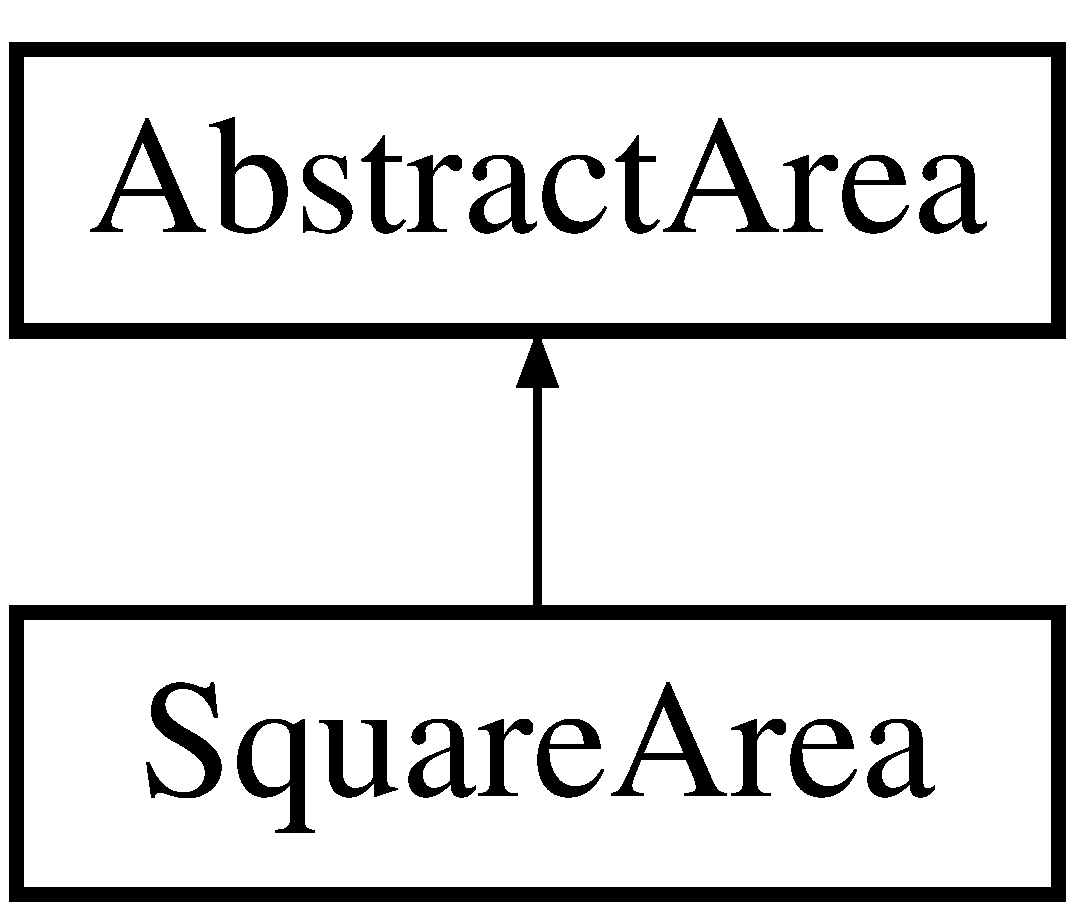
\includegraphics[height=2.000000cm]{class_abstract_area}
\end{center}
\end{figure}
\subsection*{Public Member Functions}
\begin{DoxyCompactItemize}
\item 
\mbox{\Hypertarget{class_abstract_area_a195e59e8c77d56c98dbac73febbd0adc}\label{class_abstract_area_a195e59e8c77d56c98dbac73febbd0adc}} 
virtual void {\bfseries set\+Border} (const std\+::vector$<$ double $>$ \&\+\_\+upper, const std\+::vector$<$ double $>$ \&\+\_\+lower)=0
\item 
virtual std\+::vector$<$ double $>$ \hyperlink{class_abstract_area_a832003b7c0e9e75d417c577b56a3013a}{get\+Approximation\+Inside\+Border} ()=0
\item 
virtual bool \hyperlink{class_abstract_area_a16c1ac9b2ece460e5e465cda862ce278}{is\+Out\+Of\+Border} (const std\+::vector$<$ double $>$ \&x)=0
\item 
virtual std\+::vector$<$ double $>$ \hyperlink{class_abstract_area_ab54f9d3063d994f780f2b5b67d8751d9}{get\+Upper} ()=0
\item 
virtual std\+::vector$<$ double $>$ \hyperlink{class_abstract_area_a6f5b9321813c982b37810b97c2a90257}{get\+Lower} ()=0
\item 
virtual size\+\_\+t \hyperlink{class_abstract_area_af7e07218e25ae2864d82d829ff1c10b9}{get\+Dim} ()=0
\end{DoxyCompactItemize}


\subsection{Detailed Description}
Abstract base class for area. 

\subsection{Member Function Documentation}
\mbox{\Hypertarget{class_abstract_area_a832003b7c0e9e75d417c577b56a3013a}\label{class_abstract_area_a832003b7c0e9e75d417c577b56a3013a}} 
\index{Abstract\+Area@{Abstract\+Area}!get\+Approximation\+Inside\+Border@{get\+Approximation\+Inside\+Border}}
\index{get\+Approximation\+Inside\+Border@{get\+Approximation\+Inside\+Border}!Abstract\+Area@{Abstract\+Area}}
\subsubsection{\texorpdfstring{get\+Approximation\+Inside\+Border()}{getApproximationInsideBorder()}}
{\footnotesize\ttfamily virtual std\+::vector$<$double$>$ Abstract\+Area\+::get\+Approximation\+Inside\+Border (\begin{DoxyParamCaption}{ }\end{DoxyParamCaption})\hspace{0.3cm}{\ttfamily [pure virtual]}}

Sets upper and lower bounds for Area 

Implemented in \hyperlink{class_square_area_abd7441aaf62dcbf46a22e2d6a5ef34d4}{Square\+Area}.

\mbox{\Hypertarget{class_abstract_area_af7e07218e25ae2864d82d829ff1c10b9}\label{class_abstract_area_af7e07218e25ae2864d82d829ff1c10b9}} 
\index{Abstract\+Area@{Abstract\+Area}!get\+Dim@{get\+Dim}}
\index{get\+Dim@{get\+Dim}!Abstract\+Area@{Abstract\+Area}}
\subsubsection{\texorpdfstring{get\+Dim()}{getDim()}}
{\footnotesize\ttfamily virtual size\+\_\+t Abstract\+Area\+::get\+Dim (\begin{DoxyParamCaption}{ }\end{DoxyParamCaption})\hspace{0.3cm}{\ttfamily [pure virtual]}}

Gets lower bounds of Area 

Implemented in \hyperlink{class_square_area_a4c0aafc649029e04aeffbb69d70311c5}{Square\+Area}.

\mbox{\Hypertarget{class_abstract_area_a6f5b9321813c982b37810b97c2a90257}\label{class_abstract_area_a6f5b9321813c982b37810b97c2a90257}} 
\index{Abstract\+Area@{Abstract\+Area}!get\+Lower@{get\+Lower}}
\index{get\+Lower@{get\+Lower}!Abstract\+Area@{Abstract\+Area}}
\subsubsection{\texorpdfstring{get\+Lower()}{getLower()}}
{\footnotesize\ttfamily virtual std\+::vector$<$double$>$ Abstract\+Area\+::get\+Lower (\begin{DoxyParamCaption}{ }\end{DoxyParamCaption})\hspace{0.3cm}{\ttfamily [pure virtual]}}

Gets upper bounds of Area 

Implemented in \hyperlink{class_square_area_a251a1ca1fc74129265c9d53ed508bf22}{Square\+Area}.

\mbox{\Hypertarget{class_abstract_area_ab54f9d3063d994f780f2b5b67d8751d9}\label{class_abstract_area_ab54f9d3063d994f780f2b5b67d8751d9}} 
\index{Abstract\+Area@{Abstract\+Area}!get\+Upper@{get\+Upper}}
\index{get\+Upper@{get\+Upper}!Abstract\+Area@{Abstract\+Area}}
\subsubsection{\texorpdfstring{get\+Upper()}{getUpper()}}
{\footnotesize\ttfamily virtual std\+::vector$<$double$>$ Abstract\+Area\+::get\+Upper (\begin{DoxyParamCaption}{ }\end{DoxyParamCaption})\hspace{0.3cm}{\ttfamily [pure virtual]}}

Checks if the point is out of Area 

Implemented in \hyperlink{class_square_area_ae9e9fa4d73c245d00c9bce0786fdce5c}{Square\+Area}.

\mbox{\Hypertarget{class_abstract_area_a16c1ac9b2ece460e5e465cda862ce278}\label{class_abstract_area_a16c1ac9b2ece460e5e465cda862ce278}} 
\index{Abstract\+Area@{Abstract\+Area}!is\+Out\+Of\+Border@{is\+Out\+Of\+Border}}
\index{is\+Out\+Of\+Border@{is\+Out\+Of\+Border}!Abstract\+Area@{Abstract\+Area}}
\subsubsection{\texorpdfstring{is\+Out\+Of\+Border()}{isOutOfBorder()}}
{\footnotesize\ttfamily virtual bool Abstract\+Area\+::is\+Out\+Of\+Border (\begin{DoxyParamCaption}\item[{const std\+::vector$<$ double $>$ \&}]{x }\end{DoxyParamCaption})\hspace{0.3cm}{\ttfamily [pure virtual]}}

Gets current approximation of extremum in case it steps out of Area 

Implemented in \hyperlink{class_square_area_afd99ae01cff4b1e31511a22e9b89b42a}{Square\+Area}.



The documentation for this class was generated from the following file\+:\begin{DoxyCompactItemize}
\item 
Abstract\+Area.\+h\end{DoxyCompactItemize}

\hypertarget{class_abstract_criterion}{}\section{Abstract\+Criterion Class Reference}
\label{class_abstract_criterion}\index{Abstract\+Criterion@{Abstract\+Criterion}}


Abstract base class for criterion of stopping.  




{\ttfamily \#include $<$Abstract\+Criterion.\+h$>$}

Inheritance diagram for Abstract\+Criterion\+:\begin{figure}[H]
\begin{center}
\leavevmode
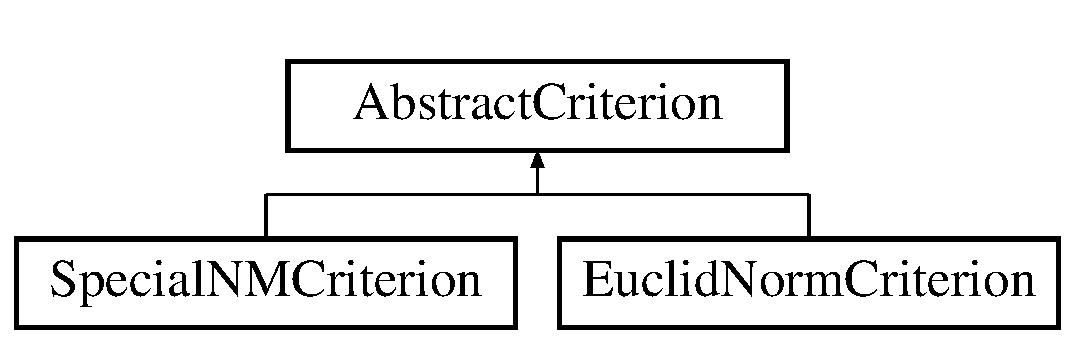
\includegraphics[height=2.000000cm]{class_abstract_criterion}
\end{center}
\end{figure}
\subsection*{Public Member Functions}
\begin{DoxyCompactItemize}
\item 
\mbox{\Hypertarget{class_abstract_criterion_a24c1c32d99515c05fdde1c851e12f83f}\label{class_abstract_criterion_a24c1c32d99515c05fdde1c851e12f83f}} 
virtual bool {\bfseries is\+Converged} (const std\+::vector$<$ double $>$ \&function) const =0
\item 
virtual bool \hyperlink{class_abstract_criterion_aa38fc5fe24aabd2b925509961eb017df}{is\+Converged} (size\+\_\+t dim, double eps, const std\+::vector$<$ double $>$ \&previous\+\_\+approximation, const std\+::vector$<$ double $>$ \&new\+\_\+approximation) const =0
\end{DoxyCompactItemize}


\subsection{Detailed Description}
Abstract base class for criterion of stopping. 

\subsection{Member Function Documentation}
\mbox{\Hypertarget{class_abstract_criterion_aa38fc5fe24aabd2b925509961eb017df}\label{class_abstract_criterion_aa38fc5fe24aabd2b925509961eb017df}} 
\index{Abstract\+Criterion@{Abstract\+Criterion}!is\+Converged@{is\+Converged}}
\index{is\+Converged@{is\+Converged}!Abstract\+Criterion@{Abstract\+Criterion}}
\subsubsection{\texorpdfstring{is\+Converged()}{isConverged()}}
{\footnotesize\ttfamily virtual bool Abstract\+Criterion\+::is\+Converged (\begin{DoxyParamCaption}\item[{size\+\_\+t}]{dim,  }\item[{double}]{eps,  }\item[{const std\+::vector$<$ double $>$ \&}]{previous\+\_\+approximation,  }\item[{const std\+::vector$<$ double $>$ \&}]{new\+\_\+approximation }\end{DoxyParamCaption}) const\hspace{0.3cm}{\ttfamily [pure virtual]}}

Checks if the current approximation is good enough based on eps-\/difference between function meanings 

Implemented in \hyperlink{class_epsilon_criterion_a3e548b8cc84db57deb00708b1c361604}{Epsilon\+Criterion}, and \hyperlink{class_euclid_norm_criterion_a210c1396bb5ba2fab199f64eea3a8f76}{Euclid\+Norm\+Criterion}.



The documentation for this class was generated from the following file\+:\begin{DoxyCompactItemize}
\item 
Abstract\+Criterion.\+h\end{DoxyCompactItemize}

\hypertarget{class_abstract_optimization_method}{}\section{Abstract\+Optimization\+Method Class Reference}
\label{class_abstract_optimization_method}\index{Abstract\+Optimization\+Method@{Abstract\+Optimization\+Method}}


Abstract base class for optimization method.  




{\ttfamily \#include $<$Abstract\+Optimization\+Method.\+h$>$}

Inheritance diagram for Abstract\+Optimization\+Method\+:\begin{figure}[H]
\begin{center}
\leavevmode
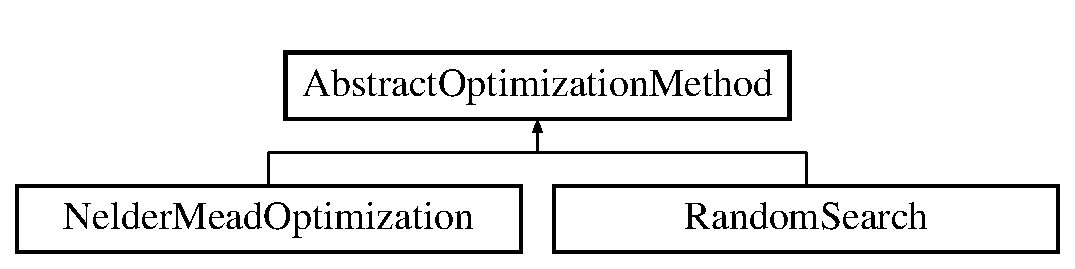
\includegraphics[height=2.000000cm]{class_abstract_optimization_method}
\end{center}
\end{figure}
\subsection*{Public Member Functions}
\begin{DoxyCompactItemize}
\item 
\mbox{\Hypertarget{class_abstract_optimization_method_ace558586052fec5b791cb90ad4f49ef6}\label{class_abstract_optimization_method_ace558586052fec5b791cb90ad4f49ef6}} 
virtual \hyperlink{class_optimization_result}{Optimization\+Result} {\bfseries optimize} (const std\+::vector$<$ double $>$ \&initial\+Approximation, const \hyperlink{class_abstract_criterion}{Abstract\+Criterion} \&criterion, const \hyperlink{class_function}{Function} \&function)=0
\end{DoxyCompactItemize}


\subsection{Detailed Description}
Abstract base class for optimization method. 

The documentation for this class was generated from the following file\+:\begin{DoxyCompactItemize}
\item 
Abstract\+Optimization\+Method.\+h\end{DoxyCompactItemize}

\hypertarget{class_epsilon_criterion}{}\section{Epsilon\+Criterion Class Reference}
\label{class_epsilon_criterion}\index{Epsilon\+Criterion@{Epsilon\+Criterion}}


Inherits from \hyperlink{class_abstract_criterion}{Abstract\+Criterion} class to implement eps-\/based stopping criterion.  




{\ttfamily \#include $<$Epsilon\+Criterion.\+h$>$}

Inheritance diagram for Epsilon\+Criterion\+:\begin{figure}[H]
\begin{center}
\leavevmode
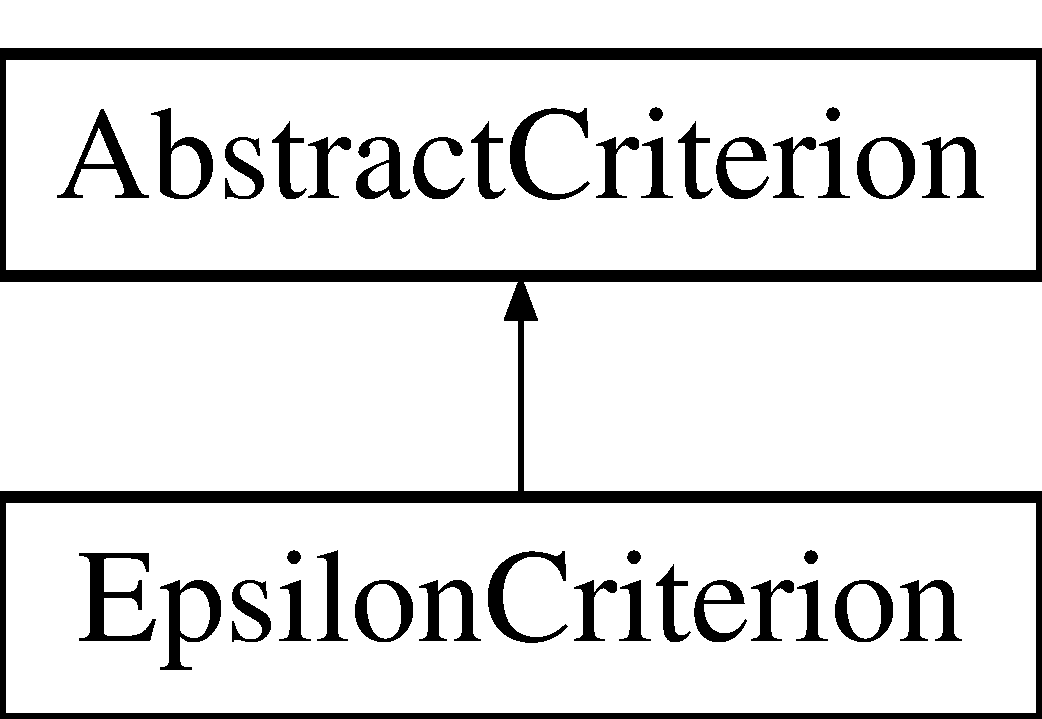
\includegraphics[height=2.000000cm]{class_epsilon_criterion}
\end{center}
\end{figure}
\subsection*{Public Member Functions}
\begin{DoxyCompactItemize}
\item 
\hyperlink{class_epsilon_criterion_a0f84f83305ad598ca5d5458de648fbc3}{Epsilon\+Criterion} (int \+\_\+n, double \+\_\+eps)
\item 
\mbox{\Hypertarget{class_epsilon_criterion_a91397b5d4bb8651a6d8f5294df39f26a}\label{class_epsilon_criterion_a91397b5d4bb8651a6d8f5294df39f26a}} 
bool {\bfseries is\+Converged} (const std\+::vector$<$ double $>$ \&function) const override
\item 
bool \hyperlink{class_epsilon_criterion_a3e548b8cc84db57deb00708b1c361604}{is\+Converged} (size\+\_\+t dim, double \hyperlink{class_epsilon_criterion_aa681adfcb498dadf5f2a5857940d535f}{eps}, const std\+::vector$<$ double $>$ \&previous\+Approximation, const std\+::vector$<$ double $>$ \&new\+Approximation) const override
\end{DoxyCompactItemize}
\subsection*{Private Attributes}
\begin{DoxyCompactItemize}
\item 
\mbox{\Hypertarget{class_epsilon_criterion_aace3bbafc317c894fb7eda51754ae0ef}\label{class_epsilon_criterion_aace3bbafc317c894fb7eda51754ae0ef}} 
const int {\bfseries dim}
\item 
const double \hyperlink{class_epsilon_criterion_aa681adfcb498dadf5f2a5857940d535f}{eps}
\end{DoxyCompactItemize}


\subsection{Detailed Description}
Inherits from \hyperlink{class_abstract_criterion}{Abstract\+Criterion} class to implement eps-\/based stopping criterion. 

\subsection{Constructor \& Destructor Documentation}
\mbox{\Hypertarget{class_epsilon_criterion_a0f84f83305ad598ca5d5458de648fbc3}\label{class_epsilon_criterion_a0f84f83305ad598ca5d5458de648fbc3}} 
\index{Epsilon\+Criterion@{Epsilon\+Criterion}!Epsilon\+Criterion@{Epsilon\+Criterion}}
\index{Epsilon\+Criterion@{Epsilon\+Criterion}!Epsilon\+Criterion@{Epsilon\+Criterion}}
\subsubsection{\texorpdfstring{Epsilon\+Criterion()}{EpsilonCriterion()}}
{\footnotesize\ttfamily Epsilon\+Criterion\+::\+Epsilon\+Criterion (\begin{DoxyParamCaption}\item[{int}]{\+\_\+n,  }\item[{double}]{\+\_\+eps }\end{DoxyParamCaption})}

Epsilon-\/const used for testing convergence 

\subsection{Member Function Documentation}
\mbox{\Hypertarget{class_epsilon_criterion_a3e548b8cc84db57deb00708b1c361604}\label{class_epsilon_criterion_a3e548b8cc84db57deb00708b1c361604}} 
\index{Epsilon\+Criterion@{Epsilon\+Criterion}!is\+Converged@{is\+Converged}}
\index{is\+Converged@{is\+Converged}!Epsilon\+Criterion@{Epsilon\+Criterion}}
\subsubsection{\texorpdfstring{is\+Converged()}{isConverged()}}
{\footnotesize\ttfamily bool Epsilon\+Criterion\+::is\+Converged (\begin{DoxyParamCaption}\item[{size\+\_\+t}]{dim,  }\item[{double}]{eps,  }\item[{const std\+::vector$<$ double $>$ \&}]{previous\+\_\+approximation,  }\item[{const std\+::vector$<$ double $>$ \&}]{new\+\_\+approximation }\end{DoxyParamCaption}) const\hspace{0.3cm}{\ttfamily [override]}, {\ttfamily [virtual]}}

Checks if the current approximation is good enough based on eps-\/difference between function meanings 

Implements \hyperlink{class_abstract_criterion_aa38fc5fe24aabd2b925509961eb017df}{Abstract\+Criterion}.



\subsection{Member Data Documentation}
\mbox{\Hypertarget{class_epsilon_criterion_aa681adfcb498dadf5f2a5857940d535f}\label{class_epsilon_criterion_aa681adfcb498dadf5f2a5857940d535f}} 
\index{Epsilon\+Criterion@{Epsilon\+Criterion}!eps@{eps}}
\index{eps@{eps}!Epsilon\+Criterion@{Epsilon\+Criterion}}
\subsubsection{\texorpdfstring{eps}{eps}}
{\footnotesize\ttfamily const double Epsilon\+Criterion\+::eps\hspace{0.3cm}{\ttfamily [private]}}

Dimension of the area 

The documentation for this class was generated from the following files\+:\begin{DoxyCompactItemize}
\item 
Epsilon\+Criterion.\+h\item 
Epsilon\+Criterion.\+cpp\end{DoxyCompactItemize}

\hypertarget{class_euclid_norm_criterion}{}\section{Euclid\+Norm\+Criterion Class Reference}
\label{class_euclid_norm_criterion}\index{Euclid\+Norm\+Criterion@{Euclid\+Norm\+Criterion}}


Inherits from \hyperlink{class_abstract_criterion}{Abstract\+Criterion} class to implement Euclid norm based stopping criterion.  




{\ttfamily \#include $<$Euclid\+Norm\+Criterion.\+h$>$}

Inheritance diagram for Euclid\+Norm\+Criterion\+:\begin{figure}[H]
\begin{center}
\leavevmode
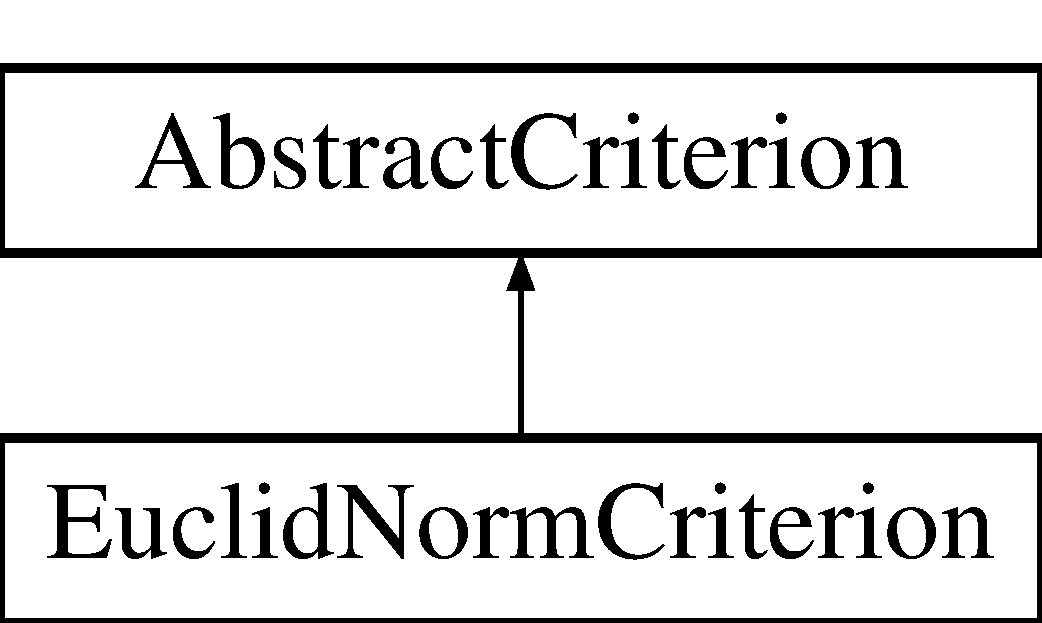
\includegraphics[height=2.000000cm]{class_euclid_norm_criterion}
\end{center}
\end{figure}
\subsection*{Public Member Functions}
\begin{DoxyCompactItemize}
\item 
\mbox{\Hypertarget{class_euclid_norm_criterion_a07b3db6194bf73995c0ca0ec17588b14}\label{class_euclid_norm_criterion_a07b3db6194bf73995c0ca0ec17588b14}} 
bool {\bfseries is\+Converged} (const std\+::vector$<$ double $>$ \&function) const override
\item 
bool \hyperlink{class_euclid_norm_criterion_a210c1396bb5ba2fab199f64eea3a8f76}{is\+Converged} (size\+\_\+t dim, double eps, const std\+::vector$<$ double $>$ \&previous\+Approximation, const std\+::vector$<$ double $>$ \&new\+Approximation) const override
\end{DoxyCompactItemize}
\subsection*{Private Attributes}
\begin{DoxyCompactItemize}
\item 
\mbox{\Hypertarget{class_euclid_norm_criterion_a9148ec33b8025fd5b656cc8222a228f7}\label{class_euclid_norm_criterion_a9148ec33b8025fd5b656cc8222a228f7}} 
const int {\bfseries M\+A\+X\+\_\+\+I\+T\+E\+R\+\_\+\+C\+O\+U\+NT} = 50000
\item 
int \hyperlink{class_euclid_norm_criterion_afbace03a4e9df12244904b3bdcf7a9e2}{iter\+Count}
\end{DoxyCompactItemize}


\subsection{Detailed Description}
Inherits from \hyperlink{class_abstract_criterion}{Abstract\+Criterion} class to implement Euclid norm based stopping criterion. 

\subsection{Member Function Documentation}
\mbox{\Hypertarget{class_euclid_norm_criterion_a210c1396bb5ba2fab199f64eea3a8f76}\label{class_euclid_norm_criterion_a210c1396bb5ba2fab199f64eea3a8f76}} 
\index{Euclid\+Norm\+Criterion@{Euclid\+Norm\+Criterion}!is\+Converged@{is\+Converged}}
\index{is\+Converged@{is\+Converged}!Euclid\+Norm\+Criterion@{Euclid\+Norm\+Criterion}}
\subsubsection{\texorpdfstring{is\+Converged()}{isConverged()}}
{\footnotesize\ttfamily bool Euclid\+Norm\+Criterion\+::is\+Converged (\begin{DoxyParamCaption}\item[{size\+\_\+t}]{dim,  }\item[{double}]{eps,  }\item[{const std\+::vector$<$ double $>$ \&}]{previous\+\_\+approximation,  }\item[{const std\+::vector$<$ double $>$ \&}]{new\+\_\+approximation }\end{DoxyParamCaption}) const\hspace{0.3cm}{\ttfamily [override]}, {\ttfamily [virtual]}}

Checks if the current approximation is good enough based on eps-\/difference between function meanings 

Implements \hyperlink{class_abstract_criterion_aa38fc5fe24aabd2b925509961eb017df}{Abstract\+Criterion}.



\subsection{Member Data Documentation}
\mbox{\Hypertarget{class_euclid_norm_criterion_afbace03a4e9df12244904b3bdcf7a9e2}\label{class_euclid_norm_criterion_afbace03a4e9df12244904b3bdcf7a9e2}} 
\index{Euclid\+Norm\+Criterion@{Euclid\+Norm\+Criterion}!iter\+Count@{iter\+Count}}
\index{iter\+Count@{iter\+Count}!Euclid\+Norm\+Criterion@{Euclid\+Norm\+Criterion}}
\subsubsection{\texorpdfstring{iter\+Count}{iterCount}}
{\footnotesize\ttfamily int Euclid\+Norm\+Criterion\+::iter\+Count\hspace{0.3cm}{\ttfamily [mutable]}, {\ttfamily [private]}}

Upper bound for probable amount of iterations for avoiding infinite looping 

The documentation for this class was generated from the following files\+:\begin{DoxyCompactItemize}
\item 
Euclid\+Norm\+Criterion.\+h\item 
Euclid\+Norm\+Criterion.\+cpp\end{DoxyCompactItemize}

\hypertarget{class_function}{}\section{Function Class Reference}
\label{class_function}\index{Function@{Function}}


Base abstract class for function definition.  




{\ttfamily \#include $<$Function.\+h$>$}

Inheritance diagram for Function\+:\begin{figure}[H]
\begin{center}
\leavevmode
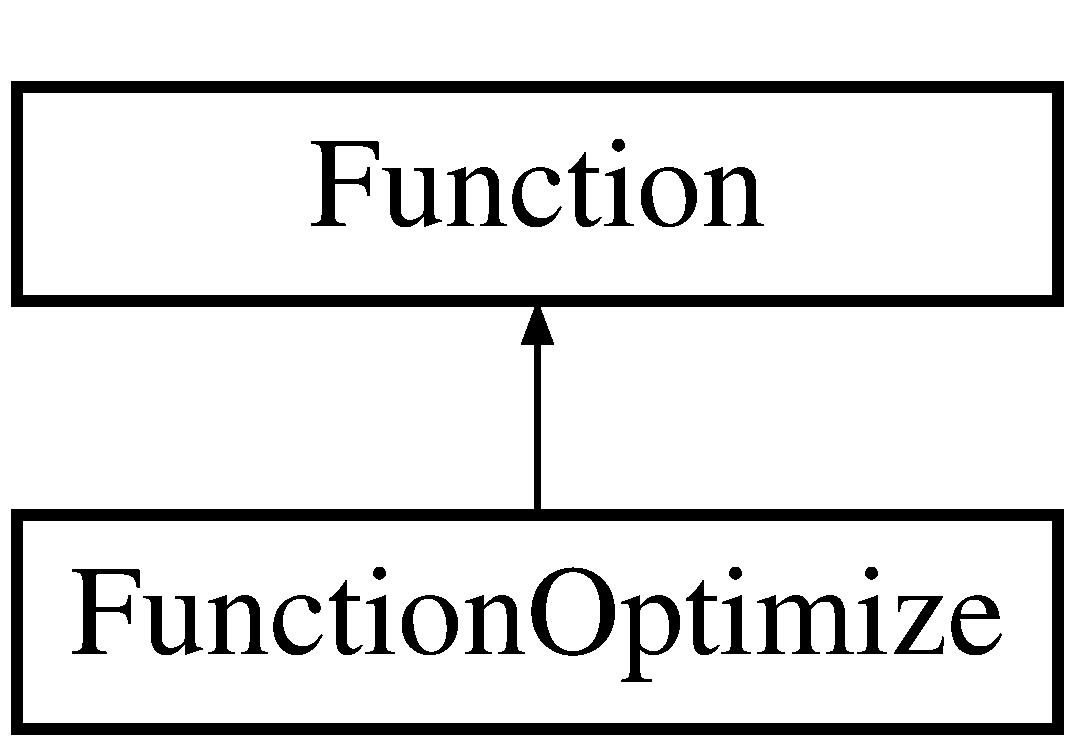
\includegraphics[height=2.000000cm]{class_function}
\end{center}
\end{figure}
\subsection*{Public Member Functions}
\begin{DoxyCompactItemize}
\item 
\mbox{\Hypertarget{class_function_adbcade5ca15e4b152bb74d4c78caaa0e}\label{class_function_adbcade5ca15e4b152bb74d4c78caaa0e}} 
virtual double {\bfseries get\+Function\+Value} (const std\+::vector$<$ double $>$ \&x) const =0
\item 
virtual \hyperlink{class_square_area}{Square\+Area} \hyperlink{class_function_add150985034ade039806b8beb9890cdc}{get\+Domain} () const =0
\end{DoxyCompactItemize}


\subsection{Detailed Description}
Base abstract class for function definition. 

\subsection{Member Function Documentation}
\mbox{\Hypertarget{class_function_add150985034ade039806b8beb9890cdc}\label{class_function_add150985034ade039806b8beb9890cdc}} 
\index{Function@{Function}!get\+Domain@{get\+Domain}}
\index{get\+Domain@{get\+Domain}!Function@{Function}}
\subsubsection{\texorpdfstring{get\+Domain()}{getDomain()}}
{\footnotesize\ttfamily virtual \hyperlink{class_square_area}{Square\+Area} Function\+::get\+Domain (\begin{DoxyParamCaption}{ }\end{DoxyParamCaption}) const\hspace{0.3cm}{\ttfamily [pure virtual]}}

Gets function value at point x 

Implemented in \hyperlink{class_function_optimize_a5b2a52f2851494a02fbd52b1862a98ae}{Function\+Optimize}.



The documentation for this class was generated from the following file\+:\begin{DoxyCompactItemize}
\item 
Function.\+h\end{DoxyCompactItemize}

\hypertarget{class_function_optimize}{}\section{Function\+Optimize Class Reference}
\label{class_function_optimize}\index{Function\+Optimize@{Function\+Optimize}}


Inherits from \hyperlink{class_function}{Function}.  




{\ttfamily \#include $<$Function\+Optimize.\+h$>$}

Inheritance diagram for Function\+Optimize\+:\begin{figure}[H]
\begin{center}
\leavevmode
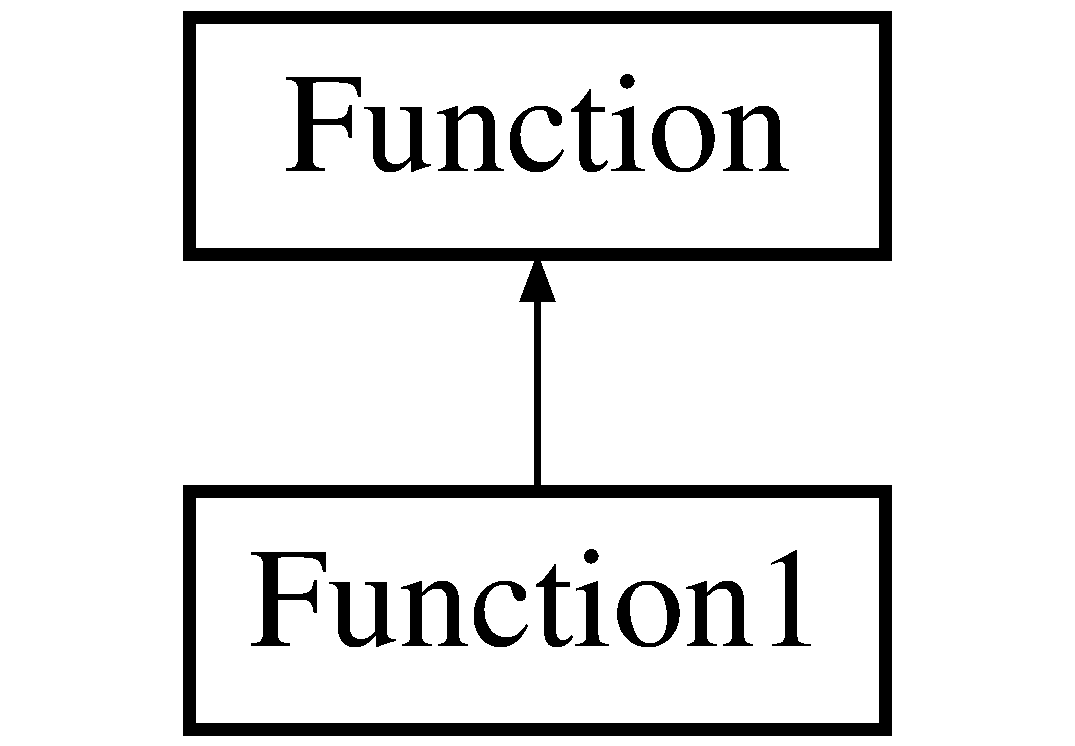
\includegraphics[height=2.000000cm]{class_function_optimize}
\end{center}
\end{figure}
\subsection*{Public Member Functions}
\begin{DoxyCompactItemize}
\item 
\mbox{\Hypertarget{class_function_optimize_a86b7d0ad4ff9ca2706cb38f7b885771b}\label{class_function_optimize_a86b7d0ad4ff9ca2706cb38f7b885771b}} 
double {\bfseries get\+Function\+Value} (const std\+::vector$<$ double $>$ \&x) const override
\item 
\mbox{\Hypertarget{class_function_optimize_a2b3d0e6b150a4418ad94bdc31b05a169}\label{class_function_optimize_a2b3d0e6b150a4418ad94bdc31b05a169}} 
{\bfseries Function\+Optimize} (int \+\_\+dim, const std\+::vector$<$ double $>$ \&upper, const std\+::vector$<$ double $>$ \&lower)
\item 
\hyperlink{class_square_area}{Square\+Area} \hyperlink{class_function_optimize_a5b2a52f2851494a02fbd52b1862a98ae}{get\+Domain} () const override
\end{DoxyCompactItemize}
\subsection*{Private Attributes}
\begin{DoxyCompactItemize}
\item 
\mbox{\Hypertarget{class_function_optimize_afb9111deb3d272e4648795e23e5271ca}\label{class_function_optimize_afb9111deb3d272e4648795e23e5271ca}} 
int {\bfseries dim}
\item 
\hyperlink{class_square_area}{Square\+Area} \hyperlink{class_function_optimize_ab3593f5f260c05abe0c7704b2356890c}{area}
\end{DoxyCompactItemize}


\subsection{Detailed Description}
Inherits from \hyperlink{class_function}{Function}. 

\subsection{Member Function Documentation}
\mbox{\Hypertarget{class_function_optimize_a5b2a52f2851494a02fbd52b1862a98ae}\label{class_function_optimize_a5b2a52f2851494a02fbd52b1862a98ae}} 
\index{Function\+Optimize@{Function\+Optimize}!get\+Domain@{get\+Domain}}
\index{get\+Domain@{get\+Domain}!Function\+Optimize@{Function\+Optimize}}
\subsubsection{\texorpdfstring{get\+Domain()}{getDomain()}}
{\footnotesize\ttfamily \hyperlink{class_square_area}{Square\+Area} Function\+Optimize\+::get\+Domain (\begin{DoxyParamCaption}{ }\end{DoxyParamCaption}) const\hspace{0.3cm}{\ttfamily [override]}, {\ttfamily [virtual]}}

Gets function value at point x 

Implements \hyperlink{class_function_add150985034ade039806b8beb9890cdc}{Function}.



\subsection{Member Data Documentation}
\mbox{\Hypertarget{class_function_optimize_ab3593f5f260c05abe0c7704b2356890c}\label{class_function_optimize_ab3593f5f260c05abe0c7704b2356890c}} 
\index{Function\+Optimize@{Function\+Optimize}!area@{area}}
\index{area@{area}!Function\+Optimize@{Function\+Optimize}}
\subsubsection{\texorpdfstring{area}{area}}
{\footnotesize\ttfamily \hyperlink{class_square_area}{Square\+Area} Function\+Optimize\+::area\hspace{0.3cm}{\ttfamily [private]}}

Dimension of the area 

The documentation for this class was generated from the following files\+:\begin{DoxyCompactItemize}
\item 
Function\+Optimize.\+h\item 
Function\+Optimize.\+cpp\end{DoxyCompactItemize}

\hypertarget{class_nelder_mead_optimization}{}\section{Nelder\+Mead\+Optimization Class Reference}
\label{class_nelder_mead_optimization}\index{Nelder\+Mead\+Optimization@{Nelder\+Mead\+Optimization}}


Inherited from Abstact\+Optimization class to present Nelder-\/\+Mead optimization.  




{\ttfamily \#include $<$Nelder\+Mead\+Optimization.\+h$>$}

Inheritance diagram for Nelder\+Mead\+Optimization\+:\begin{figure}[H]
\begin{center}
\leavevmode
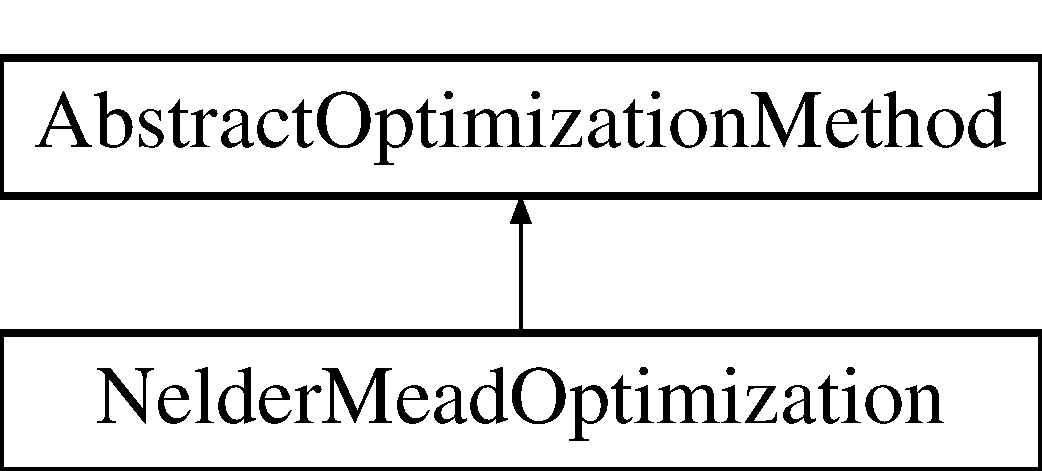
\includegraphics[height=2.000000cm]{class_nelder_mead_optimization}
\end{center}
\end{figure}
\subsection*{Public Member Functions}
\begin{DoxyCompactItemize}
\item 
\hyperlink{class_nelder_mead_optimization_a6a733eb1628525f18d098823438cbb94}{Nelder\+Mead\+Optimization} (size\+\_\+t \+\_\+dim, double \+\_\+scale)
\item 
\mbox{\Hypertarget{class_nelder_mead_optimization_a312ae6858ab89b72e77e520335524d37}\label{class_nelder_mead_optimization_a312ae6858ab89b72e77e520335524d37}} 
\hyperlink{class_optimization_result}{Optimization\+Result} {\bfseries optimize} (const std\+::vector$<$ double $>$ \&initial\+Approximation, const \hyperlink{class_abstract_criterion}{Abstract\+Criterion} \&criteria, const \hyperlink{class_function}{Function} \&function) override
\end{DoxyCompactItemize}
\subsection*{Private Attributes}
\begin{DoxyCompactItemize}
\item 
const size\+\_\+t \hyperlink{class_nelder_mead_optimization_acc80e311f32769ddbc923cd7e78718d4}{dim}
\item 
const double \hyperlink{class_nelder_mead_optimization_aadfa64f4a2f44f60755d7d40d912a53f}{scale}
\end{DoxyCompactItemize}
\subsection*{Static Private Attributes}
\begin{DoxyCompactItemize}
\item 
\mbox{\Hypertarget{class_nelder_mead_optimization_a55832ed08db34e4009e547ccbfc92f95}\label{class_nelder_mead_optimization_a55832ed08db34e4009e547ccbfc92f95}} 
static const int {\bfseries M\+A\+X\+\_\+\+IT} = 1000
\item 
static const double \hyperlink{class_nelder_mead_optimization_aa23d74cc1718065309ae6cf0daae7ae2}{A\+L\+P\+HA} = 1.\+0
\item 
static const double \hyperlink{class_nelder_mead_optimization_abcbd4c2b659649dbefe02c231b10fb2b}{B\+E\+TA} = 0.\+5
\item 
static const double \hyperlink{class_nelder_mead_optimization_a67af6800fbfe027f51fd94052b87d615}{G\+A\+M\+MA} = 2.\+0
\end{DoxyCompactItemize}


\subsection{Detailed Description}
Inherited from Abstact\+Optimization class to present Nelder-\/\+Mead optimization. 

\subsection{Constructor \& Destructor Documentation}
\mbox{\Hypertarget{class_nelder_mead_optimization_a6a733eb1628525f18d098823438cbb94}\label{class_nelder_mead_optimization_a6a733eb1628525f18d098823438cbb94}} 
\index{Nelder\+Mead\+Optimization@{Nelder\+Mead\+Optimization}!Nelder\+Mead\+Optimization@{Nelder\+Mead\+Optimization}}
\index{Nelder\+Mead\+Optimization@{Nelder\+Mead\+Optimization}!Nelder\+Mead\+Optimization@{Nelder\+Mead\+Optimization}}
\subsubsection{\texorpdfstring{Nelder\+Mead\+Optimization()}{NelderMeadOptimization()}}
{\footnotesize\ttfamily Nelder\+Mead\+Optimization\+::\+Nelder\+Mead\+Optimization (\begin{DoxyParamCaption}\item[{size\+\_\+t}]{\+\_\+dim,  }\item[{double}]{\+\_\+scale }\end{DoxyParamCaption})}

Const used for regulating simplex deformation at each step. Optimal values are chosen as default 

\subsection{Member Data Documentation}
\mbox{\Hypertarget{class_nelder_mead_optimization_aa23d74cc1718065309ae6cf0daae7ae2}\label{class_nelder_mead_optimization_aa23d74cc1718065309ae6cf0daae7ae2}} 
\index{Nelder\+Mead\+Optimization@{Nelder\+Mead\+Optimization}!A\+L\+P\+HA@{A\+L\+P\+HA}}
\index{A\+L\+P\+HA@{A\+L\+P\+HA}!Nelder\+Mead\+Optimization@{Nelder\+Mead\+Optimization}}
\subsubsection{\texorpdfstring{A\+L\+P\+HA}{ALPHA}}
{\footnotesize\ttfamily const double Nelder\+Mead\+Optimization\+::\+A\+L\+P\+HA = 1.\+0\hspace{0.3cm}{\ttfamily [static]}, {\ttfamily [private]}}

Upper bound for probable amount of iterations for avoiding infinite looping \mbox{\Hypertarget{class_nelder_mead_optimization_abcbd4c2b659649dbefe02c231b10fb2b}\label{class_nelder_mead_optimization_abcbd4c2b659649dbefe02c231b10fb2b}} 
\index{Nelder\+Mead\+Optimization@{Nelder\+Mead\+Optimization}!B\+E\+TA@{B\+E\+TA}}
\index{B\+E\+TA@{B\+E\+TA}!Nelder\+Mead\+Optimization@{Nelder\+Mead\+Optimization}}
\subsubsection{\texorpdfstring{B\+E\+TA}{BETA}}
{\footnotesize\ttfamily const double Nelder\+Mead\+Optimization\+::\+B\+E\+TA = 0.\+5\hspace{0.3cm}{\ttfamily [static]}, {\ttfamily [private]}}

Const used for regulating simplex deformation at each step. Optimal values are chosen as default \mbox{\Hypertarget{class_nelder_mead_optimization_acc80e311f32769ddbc923cd7e78718d4}\label{class_nelder_mead_optimization_acc80e311f32769ddbc923cd7e78718d4}} 
\index{Nelder\+Mead\+Optimization@{Nelder\+Mead\+Optimization}!dim@{dim}}
\index{dim@{dim}!Nelder\+Mead\+Optimization@{Nelder\+Mead\+Optimization}}
\subsubsection{\texorpdfstring{dim}{dim}}
{\footnotesize\ttfamily const size\+\_\+t Nelder\+Mead\+Optimization\+::dim\hspace{0.3cm}{\ttfamily [private]}}

Const used for regulating simplex deformation at each step. Optimal values are chosen as default \mbox{\Hypertarget{class_nelder_mead_optimization_a67af6800fbfe027f51fd94052b87d615}\label{class_nelder_mead_optimization_a67af6800fbfe027f51fd94052b87d615}} 
\index{Nelder\+Mead\+Optimization@{Nelder\+Mead\+Optimization}!G\+A\+M\+MA@{G\+A\+M\+MA}}
\index{G\+A\+M\+MA@{G\+A\+M\+MA}!Nelder\+Mead\+Optimization@{Nelder\+Mead\+Optimization}}
\subsubsection{\texorpdfstring{G\+A\+M\+MA}{GAMMA}}
{\footnotesize\ttfamily const double Nelder\+Mead\+Optimization\+::\+G\+A\+M\+MA = 2.\+0\hspace{0.3cm}{\ttfamily [static]}, {\ttfamily [private]}}

Const used for regulating simplex deformation at each step. Optimal values are chosen as default \mbox{\Hypertarget{class_nelder_mead_optimization_aadfa64f4a2f44f60755d7d40d912a53f}\label{class_nelder_mead_optimization_aadfa64f4a2f44f60755d7d40d912a53f}} 
\index{Nelder\+Mead\+Optimization@{Nelder\+Mead\+Optimization}!scale@{scale}}
\index{scale@{scale}!Nelder\+Mead\+Optimization@{Nelder\+Mead\+Optimization}}
\subsubsection{\texorpdfstring{scale}{scale}}
{\footnotesize\ttfamily const double Nelder\+Mead\+Optimization\+::scale\hspace{0.3cm}{\ttfamily [private]}}

Dimension of the area 

The documentation for this class was generated from the following files\+:\begin{DoxyCompactItemize}
\item 
Nelder\+Mead\+Optimization.\+h\item 
Nelder\+Mead\+Optimization.\+cpp\end{DoxyCompactItemize}

\hypertarget{class_optimization_result}{}\section{Optimization\+Result Class Reference}
\label{class_optimization_result}\index{Optimization\+Result@{Optimization\+Result}}


Class used for introduction of results of the optimization.  




{\ttfamily \#include $<$Optimization\+Result.\+h$>$}

\subsection*{Public Member Functions}
\begin{DoxyCompactItemize}
\item 
\mbox{\Hypertarget{class_optimization_result_a53ac4a868e151c81b9f4cd163705c351}\label{class_optimization_result_a53ac4a868e151c81b9f4cd163705c351}} 
{\bfseries Optimization\+Result} (int \+\_\+iter\+Count, int \+\_\+function\+Evaluations\+Count, const std\+::vector$<$ double $>$ \&\+\_\+minimum\+Point)
\item 
int \hyperlink{class_optimization_result_aab232c5a51fb404c8e1de38b533e617d}{get\+Iter\+Count} () const
\item 
int \hyperlink{class_optimization_result_a6f26683de442f45b95462b0dba44d737}{get\+Func\+Evaluation\+Count} () const
\item 
const std\+::vector$<$ double $>$ \& \hyperlink{class_optimization_result_a9f3d52b480c6538cd8a2da8aa127dfc8}{get\+Extr\+Point} () const
\end{DoxyCompactItemize}
\subsection*{Private Attributes}
\begin{DoxyCompactItemize}
\item 
const int \hyperlink{class_optimization_result_a2ab3b3a168bf73495f851f80d99ee3d7}{iter\+Count}
\item 
const int \hyperlink{class_optimization_result_af9b2136ff128f45202d8ad615c68cf96}{function\+Evaluations\+Count}
\item 
const std\+::vector$<$ double $>$ \hyperlink{class_optimization_result_a1d7ce65ebcdedc1d16d5365ca46d6e65}{minimum\+Point}
\end{DoxyCompactItemize}


\subsection{Detailed Description}
Class used for introduction of results of the optimization. 

\subsection{Member Function Documentation}
\mbox{\Hypertarget{class_optimization_result_a9f3d52b480c6538cd8a2da8aa127dfc8}\label{class_optimization_result_a9f3d52b480c6538cd8a2da8aa127dfc8}} 
\index{Optimization\+Result@{Optimization\+Result}!get\+Extr\+Point@{get\+Extr\+Point}}
\index{get\+Extr\+Point@{get\+Extr\+Point}!Optimization\+Result@{Optimization\+Result}}
\subsubsection{\texorpdfstring{get\+Extr\+Point()}{getExtrPoint()}}
{\footnotesize\ttfamily const std\+::vector$<$ double $>$ \& Optimization\+Result\+::get\+Extr\+Point (\begin{DoxyParamCaption}{ }\end{DoxyParamCaption}) const}

Gets general number of the function evaluations done while optimizing \mbox{\Hypertarget{class_optimization_result_a6f26683de442f45b95462b0dba44d737}\label{class_optimization_result_a6f26683de442f45b95462b0dba44d737}} 
\index{Optimization\+Result@{Optimization\+Result}!get\+Func\+Evaluation\+Count@{get\+Func\+Evaluation\+Count}}
\index{get\+Func\+Evaluation\+Count@{get\+Func\+Evaluation\+Count}!Optimization\+Result@{Optimization\+Result}}
\subsubsection{\texorpdfstring{get\+Func\+Evaluation\+Count()}{getFuncEvaluationCount()}}
{\footnotesize\ttfamily int Optimization\+Result\+::get\+Func\+Evaluation\+Count (\begin{DoxyParamCaption}{ }\end{DoxyParamCaption}) const}

Gets general number of iterations done while optimizing \mbox{\Hypertarget{class_optimization_result_aab232c5a51fb404c8e1de38b533e617d}\label{class_optimization_result_aab232c5a51fb404c8e1de38b533e617d}} 
\index{Optimization\+Result@{Optimization\+Result}!get\+Iter\+Count@{get\+Iter\+Count}}
\index{get\+Iter\+Count@{get\+Iter\+Count}!Optimization\+Result@{Optimization\+Result}}
\subsubsection{\texorpdfstring{get\+Iter\+Count()}{getIterCount()}}
{\footnotesize\ttfamily int Optimization\+Result\+::get\+Iter\+Count (\begin{DoxyParamCaption}{ }\end{DoxyParamCaption}) const}

Constructor for \hyperlink{class_optimization_result}{Optimization\+Result} class 

\subsection{Member Data Documentation}
\mbox{\Hypertarget{class_optimization_result_af9b2136ff128f45202d8ad615c68cf96}\label{class_optimization_result_af9b2136ff128f45202d8ad615c68cf96}} 
\index{Optimization\+Result@{Optimization\+Result}!function\+Evaluations\+Count@{function\+Evaluations\+Count}}
\index{function\+Evaluations\+Count@{function\+Evaluations\+Count}!Optimization\+Result@{Optimization\+Result}}
\subsubsection{\texorpdfstring{function\+Evaluations\+Count}{functionEvaluationsCount}}
{\footnotesize\ttfamily const int Optimization\+Result\+::function\+Evaluations\+Count\hspace{0.3cm}{\ttfamily [private]}}

General number of iterations \mbox{\Hypertarget{class_optimization_result_a2ab3b3a168bf73495f851f80d99ee3d7}\label{class_optimization_result_a2ab3b3a168bf73495f851f80d99ee3d7}} 
\index{Optimization\+Result@{Optimization\+Result}!iter\+Count@{iter\+Count}}
\index{iter\+Count@{iter\+Count}!Optimization\+Result@{Optimization\+Result}}
\subsubsection{\texorpdfstring{iter\+Count}{iterCount}}
{\footnotesize\ttfamily const int Optimization\+Result\+::iter\+Count\hspace{0.3cm}{\ttfamily [private]}}

Gets the point where the minimum is found at \mbox{\Hypertarget{class_optimization_result_a1d7ce65ebcdedc1d16d5365ca46d6e65}\label{class_optimization_result_a1d7ce65ebcdedc1d16d5365ca46d6e65}} 
\index{Optimization\+Result@{Optimization\+Result}!minimum\+Point@{minimum\+Point}}
\index{minimum\+Point@{minimum\+Point}!Optimization\+Result@{Optimization\+Result}}
\subsubsection{\texorpdfstring{minimum\+Point}{minimumPoint}}
{\footnotesize\ttfamily const std\+::vector$<$double$>$ Optimization\+Result\+::minimum\+Point\hspace{0.3cm}{\ttfamily [private]}}

General number of the function evaluations 

The documentation for this class was generated from the following files\+:\begin{DoxyCompactItemize}
\item 
Optimization\+Result.\+h\item 
Optimization\+Result.\+cpp\end{DoxyCompactItemize}

\hypertarget{class_random_search}{}\section{Random\+Search Class Reference}
\label{class_random_search}\index{Random\+Search@{Random\+Search}}


Inherited from \hyperlink{class_abstract_optimization_method}{Abstract\+Optimization\+Method} class. Implements random search.  




{\ttfamily \#include $<$Random\+Search.\+h$>$}

Inheritance diagram for Random\+Search\+:\begin{figure}[H]
\begin{center}
\leavevmode
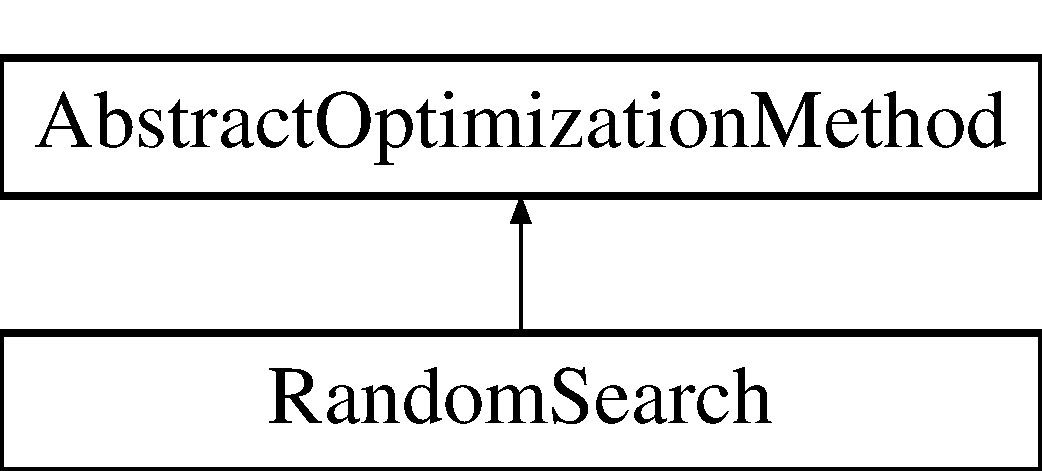
\includegraphics[height=2.000000cm]{class_random_search}
\end{center}
\end{figure}
\subsection*{Public Member Functions}
\begin{DoxyCompactItemize}
\item 
\mbox{\Hypertarget{class_random_search_aee62c84ae988d69fb05288f084415858}\label{class_random_search_aee62c84ae988d69fb05288f084415858}} 
\hyperlink{class_optimization_result}{Optimization\+Result} {\bfseries optimize} (const std\+::vector$<$ double $>$ \&initial\+Approximation, const \hyperlink{class_abstract_criterion}{Abstract\+Criterion} \&criteria, const \hyperlink{class_function}{Function} \&function) override
\item 
\mbox{\Hypertarget{class_random_search_a9d45b60cbec1268dc9087ded7cb6b450}\label{class_random_search_a9d45b60cbec1268dc9087ded7cb6b450}} 
{\bfseries Random\+Search} (double \+\_\+p)
\end{DoxyCompactItemize}
\subsection*{Private Member Functions}
\begin{DoxyCompactItemize}
\item 
std\+::vector$<$ double $>$ \hyperlink{class_random_search_a74de0911b029e12f9c02539362e39730}{get\+Random\+Point} (size\+\_\+t dim, const std\+::vector$<$ double $>$ \&upper, const std\+::vector$<$ double $>$ \&lower)
\item 
std\+::vector$<$ double $>$ \hyperlink{class_random_search_a06f28c1d7afc46a1c0382e6025e7ee4f}{sum} (const std\+::vector$<$ double $>$ \&a, const std\+::vector$<$ double $>$ \&b) const
\item 
std\+::vector$<$ double $>$ \hyperlink{class_random_search_a8a0a2518afe6d2ff29e8cb9d7b548edc}{diff} (const std\+::vector$<$ double $>$ \&a, const std\+::vector$<$ double $>$ \&b) const
\end{DoxyCompactItemize}
\subsection*{Private Attributes}
\begin{DoxyCompactItemize}
\item 
\mbox{\Hypertarget{class_random_search_a6b1a9499e9568aad8f9028f8fe04c44b}\label{class_random_search_a6b1a9499e9568aad8f9028f8fe04c44b}} 
double {\bfseries p}
\item 
std\+::mt19937 \hyperlink{class_random_search_ac78efe1a921aac4693fa32b69a2b6a98}{gen}
\item 
std\+::uniform\+\_\+real\+\_\+distribution \hyperlink{class_random_search_ad84bf71f0524d079d3e9f6f84d0a6dd7}{runif}
\end{DoxyCompactItemize}


\subsection{Detailed Description}
Inherited from \hyperlink{class_abstract_optimization_method}{Abstract\+Optimization\+Method} class. Implements random search. 

\subsection{Member Function Documentation}
\mbox{\Hypertarget{class_random_search_a8a0a2518afe6d2ff29e8cb9d7b548edc}\label{class_random_search_a8a0a2518afe6d2ff29e8cb9d7b548edc}} 
\index{Random\+Search@{Random\+Search}!diff@{diff}}
\index{diff@{diff}!Random\+Search@{Random\+Search}}
\subsubsection{\texorpdfstring{diff()}{diff()}}
{\footnotesize\ttfamily std\+::vector$<$ double $>$ Random\+Search\+::diff (\begin{DoxyParamCaption}\item[{const std\+::vector$<$ double $>$ \&}]{a,  }\item[{const std\+::vector$<$ double $>$ \&}]{b }\end{DoxyParamCaption}) const\hspace{0.3cm}{\ttfamily [private]}}

Returns componentwise sum of 2 vectors \mbox{\Hypertarget{class_random_search_a74de0911b029e12f9c02539362e39730}\label{class_random_search_a74de0911b029e12f9c02539362e39730}} 
\index{Random\+Search@{Random\+Search}!get\+Random\+Point@{get\+Random\+Point}}
\index{get\+Random\+Point@{get\+Random\+Point}!Random\+Search@{Random\+Search}}
\subsubsection{\texorpdfstring{get\+Random\+Point()}{getRandomPoint()}}
{\footnotesize\ttfamily std\+::vector$<$ double $>$ Random\+Search\+::get\+Random\+Point (\begin{DoxyParamCaption}\item[{size\+\_\+t}]{dim,  }\item[{const std\+::vector$<$ double $>$ \&}]{upper,  }\item[{const std\+::vector$<$ double $>$ \&}]{lower }\end{DoxyParamCaption})\hspace{0.3cm}{\ttfamily [private]}}

Distribution for P\+R\+NG \mbox{\Hypertarget{class_random_search_a06f28c1d7afc46a1c0382e6025e7ee4f}\label{class_random_search_a06f28c1d7afc46a1c0382e6025e7ee4f}} 
\index{Random\+Search@{Random\+Search}!sum@{sum}}
\index{sum@{sum}!Random\+Search@{Random\+Search}}
\subsubsection{\texorpdfstring{sum()}{sum()}}
{\footnotesize\ttfamily std\+::vector$<$ double $>$ Random\+Search\+::sum (\begin{DoxyParamCaption}\item[{const std\+::vector$<$ double $>$ \&}]{a,  }\item[{const std\+::vector$<$ double $>$ \&}]{b }\end{DoxyParamCaption}) const\hspace{0.3cm}{\ttfamily [private]}}

Gets random point inside the specified by bounds area 

\subsection{Member Data Documentation}
\mbox{\Hypertarget{class_random_search_ac78efe1a921aac4693fa32b69a2b6a98}\label{class_random_search_ac78efe1a921aac4693fa32b69a2b6a98}} 
\index{Random\+Search@{Random\+Search}!gen@{gen}}
\index{gen@{gen}!Random\+Search@{Random\+Search}}
\subsubsection{\texorpdfstring{gen}{gen}}
{\footnotesize\ttfamily std\+::mt19937 Random\+Search\+::gen\hspace{0.3cm}{\ttfamily [private]}}

Probability of searching in the whole area \mbox{\Hypertarget{class_random_search_ad84bf71f0524d079d3e9f6f84d0a6dd7}\label{class_random_search_ad84bf71f0524d079d3e9f6f84d0a6dd7}} 
\index{Random\+Search@{Random\+Search}!runif@{runif}}
\index{runif@{runif}!Random\+Search@{Random\+Search}}
\subsubsection{\texorpdfstring{runif}{runif}}
{\footnotesize\ttfamily std\+::uniform\+\_\+real\+\_\+distribution Random\+Search\+::runif\hspace{0.3cm}{\ttfamily [private]}}

P\+R\+NG 

The documentation for this class was generated from the following files\+:\begin{DoxyCompactItemize}
\item 
Random\+Search.\+h\item 
Random\+Search.\+cpp\end{DoxyCompactItemize}

\hypertarget{class_square_area}{}\section{Square\+Area Class Reference}
\label{class_square_area}\index{Square\+Area@{Square\+Area}}


Inherited from \hyperlink{class_abstract_area}{Abstract\+Area} class. Specifies to square area.  




{\ttfamily \#include $<$Square\+Area.\+h$>$}

Inheritance diagram for Square\+Area\+:\begin{figure}[H]
\begin{center}
\leavevmode
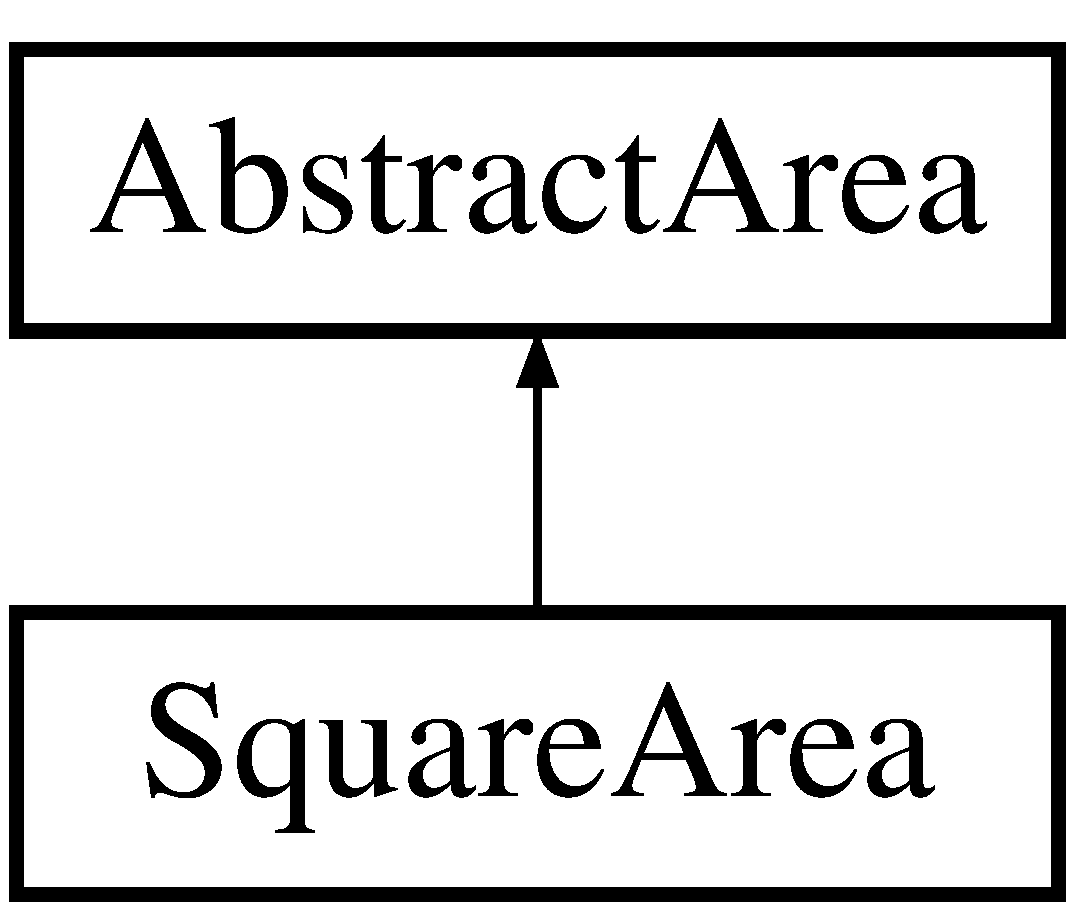
\includegraphics[height=2.000000cm]{class_square_area}
\end{center}
\end{figure}
\subsection*{Public Member Functions}
\begin{DoxyCompactItemize}
\item 
\mbox{\Hypertarget{class_square_area_aa5a2fef6a10af69f1bbf3aea7f3fc355}\label{class_square_area_aa5a2fef6a10af69f1bbf3aea7f3fc355}} 
{\bfseries Square\+Area} (size\+\_\+t \+\_\+dim)
\item 
size\+\_\+t \hyperlink{class_square_area_a4c0aafc649029e04aeffbb69d70311c5}{get\+Dim} () override
\item 
\mbox{\Hypertarget{class_square_area_aa90208b80687f7a8b6d539bc333627c9}\label{class_square_area_aa90208b80687f7a8b6d539bc333627c9}} 
void {\bfseries set\+Border} (const std\+::vector$<$ double $>$ \&\+\_\+upper, const std\+::vector$<$ double $>$ \&\+\_\+lower) override
\item 
std\+::vector$<$ double $>$ \hyperlink{class_square_area_ae9e9fa4d73c245d00c9bce0786fdce5c}{get\+Upper} () override
\item 
std\+::vector$<$ double $>$ \hyperlink{class_square_area_a251a1ca1fc74129265c9d53ed508bf22}{get\+Lower} () override
\item 
std\+::vector$<$ double $>$ \hyperlink{class_square_area_abd7441aaf62dcbf46a22e2d6a5ef34d4}{get\+Approximation\+Inside\+Border} () override
\item 
bool \hyperlink{class_square_area_afd99ae01cff4b1e31511a22e9b89b42a}{is\+Out\+Of\+Border} (const std\+::vector$<$ double $>$ \&x) override
\end{DoxyCompactItemize}
\subsection*{Private Attributes}
\begin{DoxyCompactItemize}
\item 
\mbox{\Hypertarget{class_square_area_a229fd5d084dde99c9d55e8053c482ddc}\label{class_square_area_a229fd5d084dde99c9d55e8053c482ddc}} 
std\+::vector$<$ double $>$ {\bfseries upper}
\item 
std\+::vector$<$ double $>$ \hyperlink{class_square_area_a9225f1cc2152524ea140390d605d65e0}{lower}
\item 
size\+\_\+t \hyperlink{class_square_area_ac758b2a9b3f3bd9eb0d3a0c528f23931}{dim}
\end{DoxyCompactItemize}


\subsection{Detailed Description}
Inherited from \hyperlink{class_abstract_area}{Abstract\+Area} class. Specifies to square area. 

\subsection{Member Function Documentation}
\mbox{\Hypertarget{class_square_area_abd7441aaf62dcbf46a22e2d6a5ef34d4}\label{class_square_area_abd7441aaf62dcbf46a22e2d6a5ef34d4}} 
\index{Square\+Area@{Square\+Area}!get\+Approximation\+Inside\+Border@{get\+Approximation\+Inside\+Border}}
\index{get\+Approximation\+Inside\+Border@{get\+Approximation\+Inside\+Border}!Square\+Area@{Square\+Area}}
\subsubsection{\texorpdfstring{get\+Approximation\+Inside\+Border()}{getApproximationInsideBorder()}}
{\footnotesize\ttfamily std\+::vector$<$ double $>$ Square\+Area\+::get\+Approximation\+Inside\+Border (\begin{DoxyParamCaption}{ }\end{DoxyParamCaption})\hspace{0.3cm}{\ttfamily [override]}, {\ttfamily [virtual]}}

Sets upper and lower bounds for Area 

Implements \hyperlink{class_abstract_area_a832003b7c0e9e75d417c577b56a3013a}{Abstract\+Area}.

\mbox{\Hypertarget{class_square_area_a4c0aafc649029e04aeffbb69d70311c5}\label{class_square_area_a4c0aafc649029e04aeffbb69d70311c5}} 
\index{Square\+Area@{Square\+Area}!get\+Dim@{get\+Dim}}
\index{get\+Dim@{get\+Dim}!Square\+Area@{Square\+Area}}
\subsubsection{\texorpdfstring{get\+Dim()}{getDim()}}
{\footnotesize\ttfamily size\+\_\+t Square\+Area\+::get\+Dim (\begin{DoxyParamCaption}{ }\end{DoxyParamCaption})\hspace{0.3cm}{\ttfamily [override]}, {\ttfamily [virtual]}}

Gets lower bounds of Area 

Implements \hyperlink{class_abstract_area_af7e07218e25ae2864d82d829ff1c10b9}{Abstract\+Area}.

\mbox{\Hypertarget{class_square_area_a251a1ca1fc74129265c9d53ed508bf22}\label{class_square_area_a251a1ca1fc74129265c9d53ed508bf22}} 
\index{Square\+Area@{Square\+Area}!get\+Lower@{get\+Lower}}
\index{get\+Lower@{get\+Lower}!Square\+Area@{Square\+Area}}
\subsubsection{\texorpdfstring{get\+Lower()}{getLower()}}
{\footnotesize\ttfamily std\+::vector$<$ double $>$ Square\+Area\+::get\+Lower (\begin{DoxyParamCaption}{ }\end{DoxyParamCaption})\hspace{0.3cm}{\ttfamily [override]}, {\ttfamily [virtual]}}

Gets upper bounds of Area 

Implements \hyperlink{class_abstract_area_a6f5b9321813c982b37810b97c2a90257}{Abstract\+Area}.

\mbox{\Hypertarget{class_square_area_ae9e9fa4d73c245d00c9bce0786fdce5c}\label{class_square_area_ae9e9fa4d73c245d00c9bce0786fdce5c}} 
\index{Square\+Area@{Square\+Area}!get\+Upper@{get\+Upper}}
\index{get\+Upper@{get\+Upper}!Square\+Area@{Square\+Area}}
\subsubsection{\texorpdfstring{get\+Upper()}{getUpper()}}
{\footnotesize\ttfamily std\+::vector$<$ double $>$ Square\+Area\+::get\+Upper (\begin{DoxyParamCaption}{ }\end{DoxyParamCaption})\hspace{0.3cm}{\ttfamily [override]}, {\ttfamily [virtual]}}

Sets the borders of the square domain 

Implements \hyperlink{class_abstract_area_ab54f9d3063d994f780f2b5b67d8751d9}{Abstract\+Area}.

\mbox{\Hypertarget{class_square_area_afd99ae01cff4b1e31511a22e9b89b42a}\label{class_square_area_afd99ae01cff4b1e31511a22e9b89b42a}} 
\index{Square\+Area@{Square\+Area}!is\+Out\+Of\+Border@{is\+Out\+Of\+Border}}
\index{is\+Out\+Of\+Border@{is\+Out\+Of\+Border}!Square\+Area@{Square\+Area}}
\subsubsection{\texorpdfstring{is\+Out\+Of\+Border()}{isOutOfBorder()}}
{\footnotesize\ttfamily bool Square\+Area\+::is\+Out\+Of\+Border (\begin{DoxyParamCaption}\item[{const std\+::vector$<$ double $>$ \&}]{x }\end{DoxyParamCaption})\hspace{0.3cm}{\ttfamily [override]}, {\ttfamily [virtual]}}

Gets current approximation of extremum in case it steps out of Area 

Implements \hyperlink{class_abstract_area_a16c1ac9b2ece460e5e465cda862ce278}{Abstract\+Area}.



\subsection{Member Data Documentation}
\mbox{\Hypertarget{class_square_area_ac758b2a9b3f3bd9eb0d3a0c528f23931}\label{class_square_area_ac758b2a9b3f3bd9eb0d3a0c528f23931}} 
\index{Square\+Area@{Square\+Area}!dim@{dim}}
\index{dim@{dim}!Square\+Area@{Square\+Area}}
\subsubsection{\texorpdfstring{dim}{dim}}
{\footnotesize\ttfamily size\+\_\+t Square\+Area\+::dim\hspace{0.3cm}{\ttfamily [private]}}

Lower bound of the area \mbox{\Hypertarget{class_square_area_a9225f1cc2152524ea140390d605d65e0}\label{class_square_area_a9225f1cc2152524ea140390d605d65e0}} 
\index{Square\+Area@{Square\+Area}!lower@{lower}}
\index{lower@{lower}!Square\+Area@{Square\+Area}}
\subsubsection{\texorpdfstring{lower}{lower}}
{\footnotesize\ttfamily std\+::vector$<$double$>$ Square\+Area\+::lower\hspace{0.3cm}{\ttfamily [private]}}

Upper bound of the area 

The documentation for this class was generated from the following files\+:\begin{DoxyCompactItemize}
\item 
Square\+Area.\+h\item 
Square\+Area.\+cpp\end{DoxyCompactItemize}

%--- End generated contents ---

% Index
\backmatter
\newpage
\phantomsection
\clearemptydoublepage
\addcontentsline{toc}{chapter}{Index}
\printindex

\end{document}
